\documentclass[palatino, nochap]{apuntes}

\title{Diseño y análisis de algoritmos - Resumen}
\author{Guillermo Julián Moreno}
\date{15/16 C1}

% Paquetes adicionales
\usepackage{minted}
\usepackage{fancysprefs}
\usepackage{tree}
\usepackage{tikz-qtree}
\usepackage{wrapfig}

% --------------------

\begin{document}
\pagestyle{plain}
\maketitle

\tableofcontents
\newpage

\section{Grafos}

Suponemos un cierto conocimiento básico sobre grafos. Denotaremos los grafo por $G = (V,E)$, con $V$ el conjunto de vértices o nodos y $E$ las aristas, donde $(u,v)$ con $u,v ∈ V$ es una arista que, en grafos dirigidos, implica dirección $u \to v$. Si el grafo es ponderado, los ejes tienen peso $w_{uv}$.

\subsection{Distancia mínima}

El problema se plantea fácilmente: dado un grafo $G$ y dos vértices $u$ y $v$, encontrar un camino mínimo $π = \set{u \equiv u_0, u_1, \dotsc, u_k \equiv v}$ de uno a otro.


\begin{listing}[hbtp]
\begin{minted}[frame=lines, fontsize=\scriptsize, tabsize=4]{python}
def dijkstra(G, from, costs, adjacent_nodes):
	n_nodes = len(G)
	visited = [False] * n_nodes
	path = [-1] * n_nodes
	distance = [infinity] * n_nodes
	queue = PriorityQueue()

	distance[from] = 0
	queue.put(from, priority = 0)

	while not q.empty():
		priority, node = queue.get()

		if not visited[node]:
			visited[node] = True

			for adj in adjacent_nodes[node]:
				if distance[adj] > distance[node] + costs[node, adj]:
					# Actualizamos el coste y el camino al nodo adyacente
					distance[adj] = distance[node] + costs[node, adj]
					path[adj] = node
					q.put(adj, priority = distance[adj])

	return path, distances
\end{minted}
\caption{Algoritmo de Dijkstra para encontrar los caminos mínimos a todos los nodos de un grafo $G$ dado un nodo incial.}
\label{lst:Dijkstra}
\end{listing}

Si el grafo no es ponderado, con una búsqueda en anchura (BFS) nos valdrá. Ahora bien, la cosa se complica en grafos ponderados. Para ello necesitaremos el \concept{Algoritmo\IS de Dijkstra} (\fref{lst:Dijkstra}), que usa una BFS con cola de prioridad. La prioridad de cada nodo es su distancia al nodo origen: cuanta menor es esa distancia, antes lo visitamos.

El coste de Dijkstra es $O(\abs{V} + \abs{E} \log \abs{V})$. Como explicación rápida, tenemos como mucho $\abs{E}$ aristas a meter en la cola de prioridad, que tendrá coste de inserción y extracción $O(\log \abs{E})$. Tenemos que recorrer todas las aristas, así que tendremos en total unas $O(\abs{E} \log \abs{E})$ operaciones. Como $\abs{E} = O(\abs{V}^2)$, lo que nos queda asintóticamente es $O(\abs{V} + \abs{E}\log \abs{V})$.

Cuando lo que queremos es buscar los caminos mínimos entre todos los pares de nodos, podemos usar un algoritmo algo mejor, especialmente para grafos densos donde el coste de Dijkstra iterado se va a $O(\abs{V}^3 \log \abs{V})$. Lo que usaremos en este caso será el \concept{Algoritmo\IS de Floyd-Warshall} (\fref{lst:FloydWarshall}), que tiene coste $O(\abs{V}^3)$.

\begin{listing}[hbtp]
\begin{minted}[frame=lines, fontsize=\scriptsize, tabsize=4]{python}

def floydWarshall(G):
	n_nodes = len(G)
	min_distances = G # Suponemos G dado como matriz.

	for k in range(node_count):
		for i in range(node_count):
			for j in range(node_count):
				if min_distances[i][j] > min_distances[i][k] + min_distances[k][j]:
					min_distances[i][j] = min_distances[i][k] + min_distances[k][j]

	return min_distances
\end{minted}
\caption{Algoritmo de Floyd-Warshall para encontrar todos los caminos mínimos entre los nodos de un grafo.}
\label{lst:FloydWarshall}
\end{listing}

\subsection{Árboles abarcadores}

La idea de un árbol abarcador es quedarnos con sólo un subconjunto $E_T ⊆ E$ de las aristas de un grafo, de tal forma que tengamos un árbol con todos los nodos del grafo original. BFS y DFS nos permiten generar estos árboles abarcadores, aunque querremos algo más sofisticado para sacar árboles con propiedades más específicas.

Por ejemplo, buscaremos árboles abarcadores mínimos, esto es, árboles $T = (V, E_T)$ tales que, para cualquier otro árbol abarcador $T' = (V, E_{T'})$, la suma de costes de las aristas $E_T$ sea menor que la de los costes de $E_{T'}$.

Un algoritmo para encontrar un árbol abarcador mínimo es el \concept{Algoritmo\IS de Prim} (\fref{lst:Prim}), que en el fondo no es más que una modificación ligera de Dijkstra en el que en lugar de mantener la tabla de distancias mantenemos una tabla de costes para cada arista del árbol. El coste de Prim es el mismo que el de Dijkstra, $O(\abs{E} \log \abs{V})$.


\begin{listing}[hbtp]
\begin{minted}[frame=lines, fontsize=\scriptsize, tabsize=4]{python}
def dijkstra(G, from, costs, adjacent_nodes):
	n_nodes = len(G)
	visited = [False] * n_nodes
	path = [-1] * n_nodes
	tree_costs = [infinity] * n_nodes
	queue = PriorityQueue()

	tree_costs[from] = 0
	queue.put(from, priority = 0)

	while not q.empty():
		priority, node = queue.get()

		if not visited[node]:
			visited[node] = True

			for adj in adjacent_nodes[node]:
				if tree_costs[adj] > costs[node, adj]
					# Actualizamos el coste y el camino al nodo adyacente
					tree_costs[adj] = costs[node, adj]
					path[adj] = node
					q.put(adj, priority = tree_costs[adj])

	return path, tree_costs
\end{minted}
\caption{Algoritmo de Prim para encontrar un árbol abarcador mínimo. El árbol se reconstruye recorriendo el array \texttt{path}: el nodo padre de $u$ es \texttt{path[u]} y la arista que los conecta tiene coste \texttt{tree\_costs[u]}.}
\label{lst:Prim}
\end{listing}

El otro algoritmo posible es el \concept{Algoritmo\IS de Kruskal}, probablemente más intuitivo. Se crea un bosque, al que por cada nodo se añade un árbol que consta únicamente de ese nodo. Después, se itera por cada rama, empezando por las de menor peso. Cada rama conecta dos nodos: si podemos (esto es, la rama no genera ciclos o, equivalentemente, los nodos están en árboles distintos), construimos un nuevo árbol uniendo los árboles en los que está cada nodo con la rama que consideramos. Al final nos quedará un único árbol (si no, es que el grafo no era conexo).

Para implementar el algoritmo (no vamos a poner el pseudocódigo) creamos un tipo abstracto de datos que representa la partición del conjunto de vértices $V$ y que nos permita realizar uniones de conjuntos.

Lo bueno es que un conjunto se puede representar por un árbol. A cada conjunto se le asigna un representante $u$, que consideraremos la raíz del árbol. Cada vértice del árbol es un elemento de ese conjunto. Unir dos árboles representados por elementos $u$ e $u$ será tan sencillo como hacer que $u$ sea un nodo hijo de $u$.

Así, podremos representar la partición por una matriz \texttt{p}, donde \texttt{p[u]} es el nodo padre de $u$ o, si $u$ es nodo raíz, valdrá $-1$. Luego todo esto se puede hacer más eficiente para que el coste de las uniones y de la búsqueda de un representante sea menor.

El algoritmo de Kruskal tiene coste $O(\abs{E} \log \abs{V})$ por las operaciones con la cola de prioridad.

\subsubsection{Invariantes de bucle}

Tanto Prim como Kruskal tienen una cosa en común: hay una condición que siempre se cumple tras cada iteración, que es que las aristas seleccionadas forman parte de un árbol abarcador mínimo. Esta condición se llama una \concept{Invariante\IS de bucle} y dan una idea de la corrección de algoritmos iterativos.

\subsection{Conexión en grafos}

\begin{wrapfigure}{r}{0.35\textwidth}
\centering
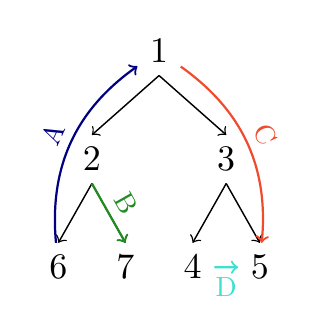
\begin{tikzpicture}[scale=1.3]
\tikzset{sibling distance=7pt}
\tikzset{edge from parent/.append style={->}}
\Tree [.\node(1) {1};
	[.\node(2) {2};
		[.\node (6) {6}; ]
		[.\node (7) {7}; ] ]
	[.3
		[.\node(4) {4}; ]
		[.\node(5) {5}; ] ]
]

\draw[NavyBlue, thick, ->] (6) to[bend left] node[midway, sloped, above] {A} (1);
\draw[ForestGreen, thick, ->] (2.south) to node[midway, sloped, above] {B} (7.north);
\draw[RedOrange, thick, ->] (1) to[bend left] node[midway, sloped, above] {C} (5);
\draw[Turquoise, thick, ->] (4) to node[midway, sloped, below] {D} (5);
\end{tikzpicture}
\caption{DFS induce una clasificación de las aristas de un grafo según cómo queden en el árbol.}
\label{fig:ArbolDFS}
\end{wrapfigure}

Para estudiar la conexión en grafos, se utilizan algoritmos derivados de la búsqueda en profundidad o DFS. Una de las primeras cosas que podemos ver es que las aristas $(u,v)$ se pueden clasificar según cómo queden en el árbol que genera DFS (\fref{fig:ArbolDFS}):

\begin{itemize}
\item \concept{Arista\IS árbol}: Aristas tipo B, donde $v$ es nodo hijo de $u$.
\item \concept{Arista\IS ascendentes}: Aristas tipo A, donde podemos llegar de $v$ a $u$ subiendo por el árbol.
\item \concept{Arista\IS descendentes}: Aristas tipo C, donde podemos llegar de $v$ a $u$ bajando por el árbol.
\item \concept{Arista\IS cruzada}: Aristas tipo D, básicamente cualquier otra que no quepa en la anterior clasificación.
\end{itemize}

En grafos no dirigidos, las aristas ascendentes y descendentes son iguales. Además, en ese caso tampoco hay aristas cruzadas (si queremos ir a un nodo que ya esté en el grafo, lo hemos visitado y por lo tanto DFS no pasará por ahí). La idea de esto viene de un teorema\footnote{Que por lo obvio que es no debería llamarse teorema ni de lejos.}, llamado \concept{Teorema\IS del paréntesis}. Si llevamos un conteo $c$ de cuántos nodos hemos visitado, y llamamos $d_u$ y $f_u$ al valor de $c$ cuando DFS llega y sale de $u$ respectivamente, la visita posterior a un nodo $v$ hijo de $u$ habrá empezado después que $d_u$ y terminado antes que $f_u$. Si no es un nodo hijo, entonces $f_u < d_u$. En otras palabras, si llamamos $I_u = (d_u, f_u)$ y $I_v = (d_v, f_v)$ con $d_u < d_v$, entonces \[ I_v ⊂ I_u \text{ ó bien } I_u ∩ I_v = ∅ \]

Al estudiar conexión, querremos estudiar componentes y ver cuáles son los \concept{Puntos\IS de articulación}, esto es, nodos que si se quitan del grafo nos queda un grafo no conexo. Obviamente, esta definición sólo vale si el grafo es conexo: si no, no tiene demasiado sentido. Un grafo no dirigido sin puntos de articulación es un \concept{Grafo\IS biconexo}.

Para encontrar los puntos de articulación de un grafo, ejecutamos DFS sobre el grafo. Un nodo $u$ será un punto de articulación si existe un hijo $v$ de $u$ que no tenga una arista ascendente a algún antecesor de $u$. Eso se traduce en cosas.

\subsection{Grafos dirigidos acíclicos}

Pasamos a estudiar ahora los grafos dirigidos acíclicos (DAG). Siguiendo con la clasificación de aristas de la sección anterior, es fácil ver que son los que el DFS no nos da aristas ascendentes.

Un algoritmo interesante en estos grafos es el \concept{Ordenamiento\IS topológico} o \textit{toposort}, que nos va a dar una ordenación $≤$ de los nodos tal que si $(u,v)$ es un eje, entonces $u ≤ v$. Esta ordenación se puede obtener con una lista vinculada y DFS: cuando DFS acaba de visitar un nodo $u$, éste se añade al principio de la lista. Así, se garantiza que todos los nodos a los que se puede llegar en un salto desde $u$ están después que $u$.

Esta ordenación nos permitirá, por ejemplo, encontrar caminos mínimos en un grafo en tiempo lineal



\begin{listing}[hbtp]
\begin{minted}[frame=lines, fontsize=\scriptsize, tabsize=4]{python}
def shortestPathsDAG(G, from, cost, adjacent_nodes):
	n_nodes = len(G)
	parent = [-1] * n_nodes
	distance = [infinity] * n_nodes
	nodes = toposort(G) # Lista ordenada de menor a mayor de los nodos de G

	distance[from] = 0

	for node in nodes:
		for adj in adjacent_nodes[node]:
			if distance[adj] > distance[node] + cost[node, adj]:
				distance[adj] = distance[node] + cost[node, adj]
				parent[adj] = node

	return distance, parent
\end{minted}
\caption{Algoritmo de distancias mínimas para grafos dirigidos acíclicos usando una ordenación topológica. La ventaja es que sólo podemos llegar de un nodo a los que están detrás en la lista, así que tenemos una forma de recorrer la lista de nodos más simple que en otros algoritmos de caminos mínimos.}
\label{lst:Prim}
\end{listing}

\appendix

\printindex
\end{document}
